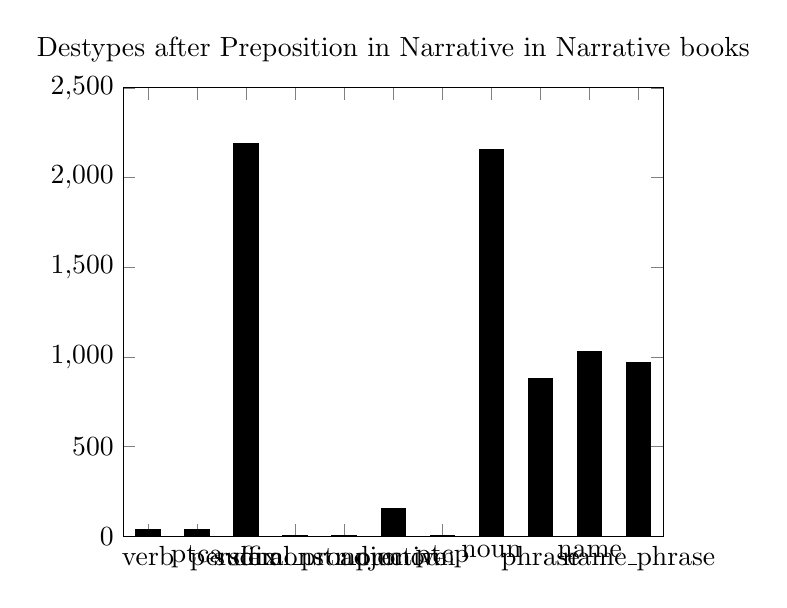
\begin{tikzpicture}[baseline]
\begin{axis}[
title = Destypes after Preposition in Narrative in Narrative books,
xmin=-0.5, xmax=10.5,
ymin=0, ymax=2500,
xtick={0,1,2,3,4,5,6,7,8,9,10},
xticklabels={verb,ptca,suffix,personal\_pronoun,demonstr\_pronoun,adjective,ptcp,noun,phrase,name,name\_phrase},
xticklabel style = {\xticklabel},
]
\draw[draw=\bardrawcolor,fill=\barcolor] (axis cs:-0.25,0) rectangle (axis cs:0.25,39);
\draw[draw=\bardrawcolor,fill=\barcolor] (axis cs:0.75,0) rectangle (axis cs:1.25,37);
\draw[draw=\bardrawcolor,fill=\barcolor] (axis cs:1.75,0) rectangle (axis cs:2.25,2188);
\draw[draw=\bardrawcolor,fill=\barcolor] (axis cs:2.75,0) rectangle (axis cs:3.25,1);
\draw[draw=\bardrawcolor,fill=\barcolor] (axis cs:3.75,0) rectangle (axis cs:4.25,5);
\draw[draw=\bardrawcolor,fill=\barcolor] (axis cs:4.75,0) rectangle (axis cs:5.25,154);
\draw[draw=\bardrawcolor,fill=\barcolor] (axis cs:5.75,0) rectangle (axis cs:6.25,4);
\draw[draw=\bardrawcolor,fill=\barcolor] (axis cs:6.75,0) rectangle (axis cs:7.25,2158);
\draw[draw=\bardrawcolor,fill=\barcolor] (axis cs:7.75,0) rectangle (axis cs:8.25,878);
\draw[draw=\bardrawcolor,fill=\barcolor] (axis cs:8.75,0) rectangle (axis cs:9.25,1032);
\draw[draw=\bardrawcolor,fill=\barcolor] (axis cs:9.75,0) rectangle (axis cs:10.25,970);
\end{axis}
\end{tikzpicture}

